\section{Results}
\label{sec:results}
To evaluate GBD as a viable physical optics propagation technique we benchmark its performance versus traditional diffraction simulations for a given observatory coupled to a vortex coronagraph. The fiducial observatory used in this study is a Ritchey-Chretien (RCs) objective based on the Hubble Space Telescope (HST) using an unobscured aperture. This model is constructed in Zemax OpticStudio, using the system prescription is given in Table \ref{tab:fiducial_observatory_specs} and is illustrated in Figure \ref{fig:telescope_model}.

\begin{table}[H]
    \centering
    \begin{tabular}{c c c c c}
        \hline
        Surface & RoC [m] & Conic Constant & Distance [m] & Diameter [m]  \\
        \hline
        M1 & -11.0400 & -1.00230 & -4.90607 & 2.40000 \\
        M2 & 1.35800 & -1.49686 &  6.40620 & 0.28112 \\
        \hline
        \\
    \end{tabular}
    \caption{Optical system prescription for the RC telescope based on the HST used in this investigation. All distances are given in meters. RoC stands for Radius of Curvature, and the sign convention is chosen such that negative values are concave, and positive values are convex.}
    \label{tab:fiducial_observatory_specs}
\end{table}

\begin{figure}[H]
    \centering
    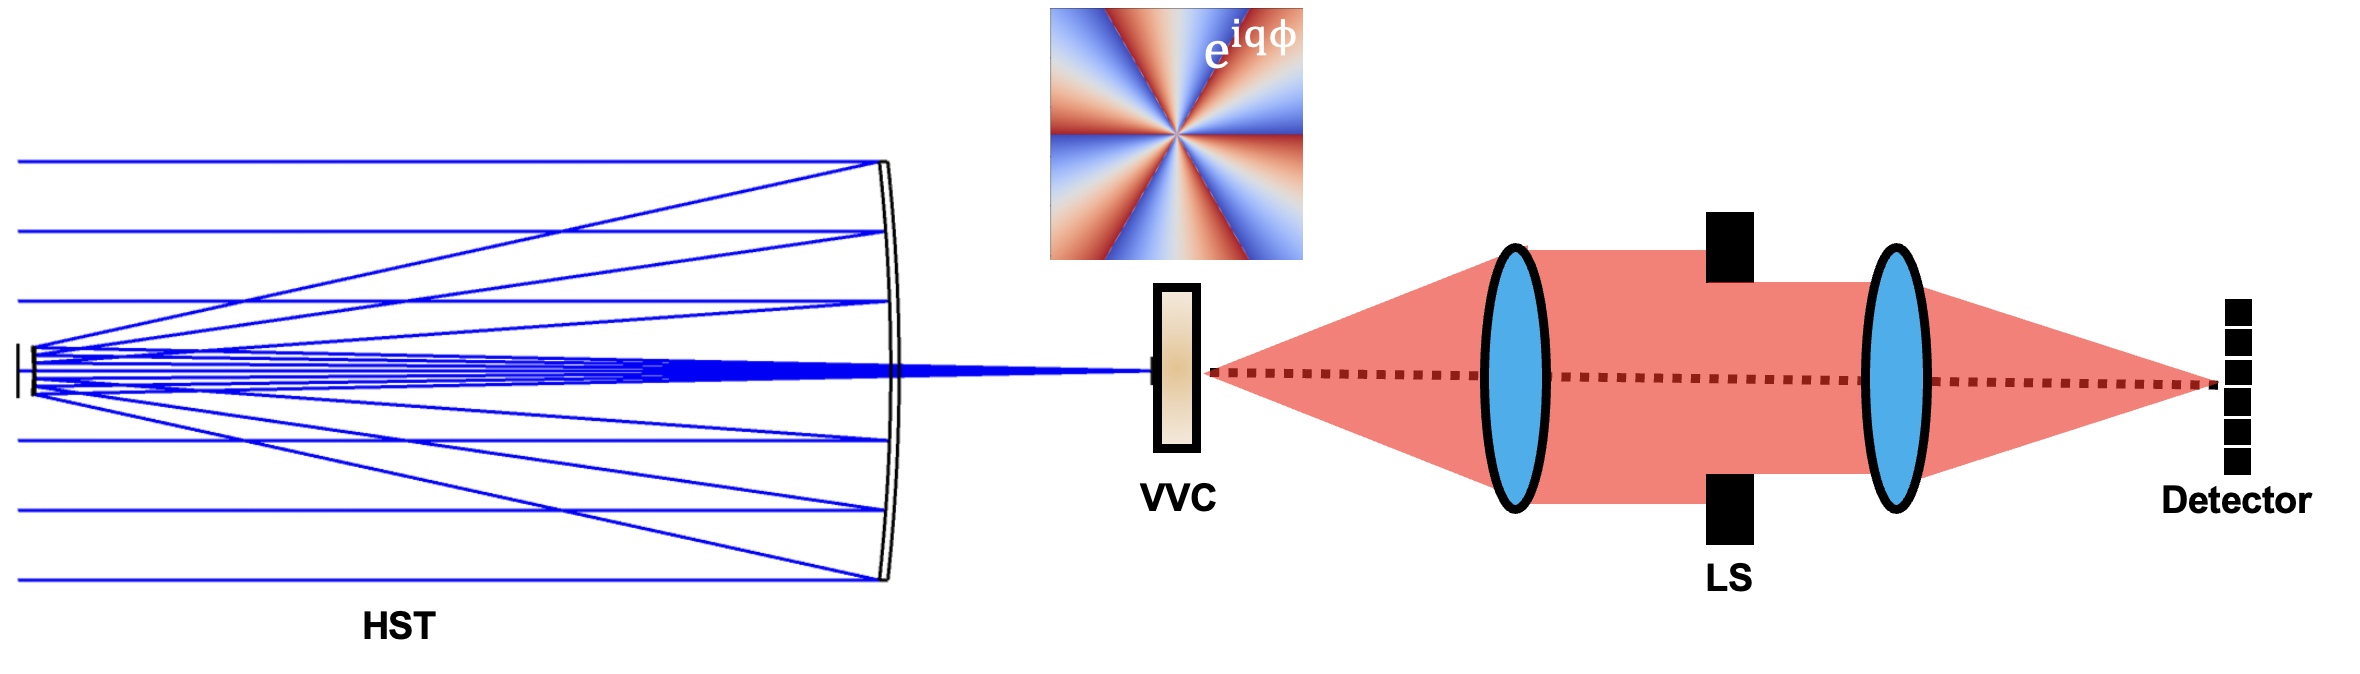
\includegraphics[width=\textwidth]{telescope_model.png}
    \caption{Illustration of the hybrid propagation physics model used to produce the results in this Section. The system prescription in Table \ref{tab:fiducial_observatory_specs} is loaded into Zemax OpticStudio and shown on the left (labeled HST). The phase of a vortex coronagraph (VVC) is shown in the middle. The GBD PSF is computed at this plane and propagated through the coronagraph using HCIPy to arrive at the final image at the detector plane.}
    \label{fig:telescope_model}
\end{figure}

We first compare the PSFs generated by GBD to the analytical Airy function to assess the degree to which GBD can represent the focused field after a circular aperture. We then compare an aberrated GBD PSF to one produced by the Zemax Huygens PSF analysis tool to assess GBD's ability to reconstruct the field after a vignetted and aberrated wavefront. Finally, we propagate the focused field after a circular aperture produced by GBD through a Fraunhofer model of a vortex coronagraph and compare it to the results given by using solely Fraunhofer diffraction. The PSF simulations conducted in Section 4.2 are monochromatic simulations at 1.65 $\mu$m on a detector with 256 $\times$ 256 pixels over 1 $\times$ 1 mm (or 25 $\times$ 25 $\frac{\lambda}{D}$ ). The coronagraph simulations conducted in Section 4.3 are conducted at the same wavelength, but with 1600 $\times$ 1600 pixels across 8 $\times$ 8 mm (or 200 $\times$ 200 $\frac{\lambda}{D}$) to better sample the vortex mask and reach the desired contrast levels for both the Hybrid and Fraunhofer model.

\subsection{The Fiducial Coronagraph}
Our goal in this study is to assess the feasibility of GBD to integrate ray models of observatories into physical optics models of coronagraphs accurately. To quantify this, we propagate the images produced by GBD and the analytical Airy function through a charge-2 vortex coronagraph (VC) \cite{mawet_annular_2005,lee_experimental_2006}. The optical VC is the general case of the vector vortex coronagraph\cite{mawet_vector_2010} which has shown great promise for future missions to image Earthlike exoplanets \cite{serabyn_vector_2019-1}. These coronagraphs are excellent at rejecting low-order spatial modes, while transmitting the remainder of the light. We expect that traditional GBD will have some difficulty in accurately modeling high-spatial frequency content, and that it will manifest in the focal plane of this fiducial coronagraph if the error is limiting. If not, then we can conclude that GBD is suitable for high-contrast imaging simulation.

The complex amplitude of the charge-$q$ VC focal plane mask is given by
\begin{equation}
	U(x,y) = exp\Bigl[i q \arctan(\frac{y}{x})\Bigr],
	\label{eq:vortex}
\end{equation}
where $q$ is the topological charge and the transmission is unity everywhere except for the center pixel, where it is 0. This is because there is a singularity in the phase ramp at this location, so it must be masked out. We chose the VC because of its ability to effectively reject on-axis starlight at a given wavelength. Should GBD introduce undesirable artifacts into the PSF, it should be visible in the coronagraph focal plane. Modeling a VC accurately is challenging computationally, because the on-axis starlight is only completely rejected if the focal plane is infinitely sampled. The singularity at the center must also be sampled highly in order to accurately sample the rapid change in phase immediately around it without discretization errors. These require very large arrays ($\ge$ 16k $\times$ 16k arrays) for meaningful starlight rejection, which considerably slows the simulation. To overcome this computational burden, a multi-step propagation algorithm can be used to sample the central singularity higher than the rest of the field. HCIPy\cite{por2018hcipy} has this algorithm implemented in the \verb"VortexCoronagraph" class, which accepts a user-specified wavefront and then outputs the wavefront after the VC and before the Lyot stop. We can define our GBD PSF as an HCIPy wavefront and propagate it through the coronagraph to complete our hybrid propagation model and analyze the image plane residuals. We can then compare the residuals of our hybrid propagation model to one where the PSF of a circular aperture was computed with Fraunhofer diffraction. This permits us to compare the scale of the error introduced by the hybrid propagation model against the numerical simulation errors present in traditional diffraction simulation.

\label{sect:results}  % \label{} allows reference to this 

\subsection{The Observatory PSF}
First we examine GBD's ability to construct the Airy pattern. The Airy pattern represents the ``ideal" diffraction-limited observatory image for a circular aperture. The analytical solution for this image is known and available in POPPY, so we have a point of comparison that is not limited by numerical simulation errors. Shown in Figures \ref{fig:airy_even} and \ref{fig:airy_fib} are the PSF simulations generated by GBD using the even and Fibonacci sampling schemes. We also plot a comparison of the Modulation Transfer Function (MTF) to better illustrate how the transfer of individual spatial frequencies is affected by GBD. An important parameter in these simulations was the degree to which the effective diameter of the entrance pupil was appropriately captured. In Figures \ref{fig:gbd_essentials}c-d, we observe that GBD results in some energy spillover outside of the original aperture function, which would result in a PSF with an incorrect spatial extent. To mitigate this effect, we remove any beamlets within half a waist radius of the aperture boundary. This is a trade-off between too much energy outside of the aperture which results in a smaller PSF, and too little energy within the aperture which results in a larger PSF.

\begin{figure}[H]
    \centering
    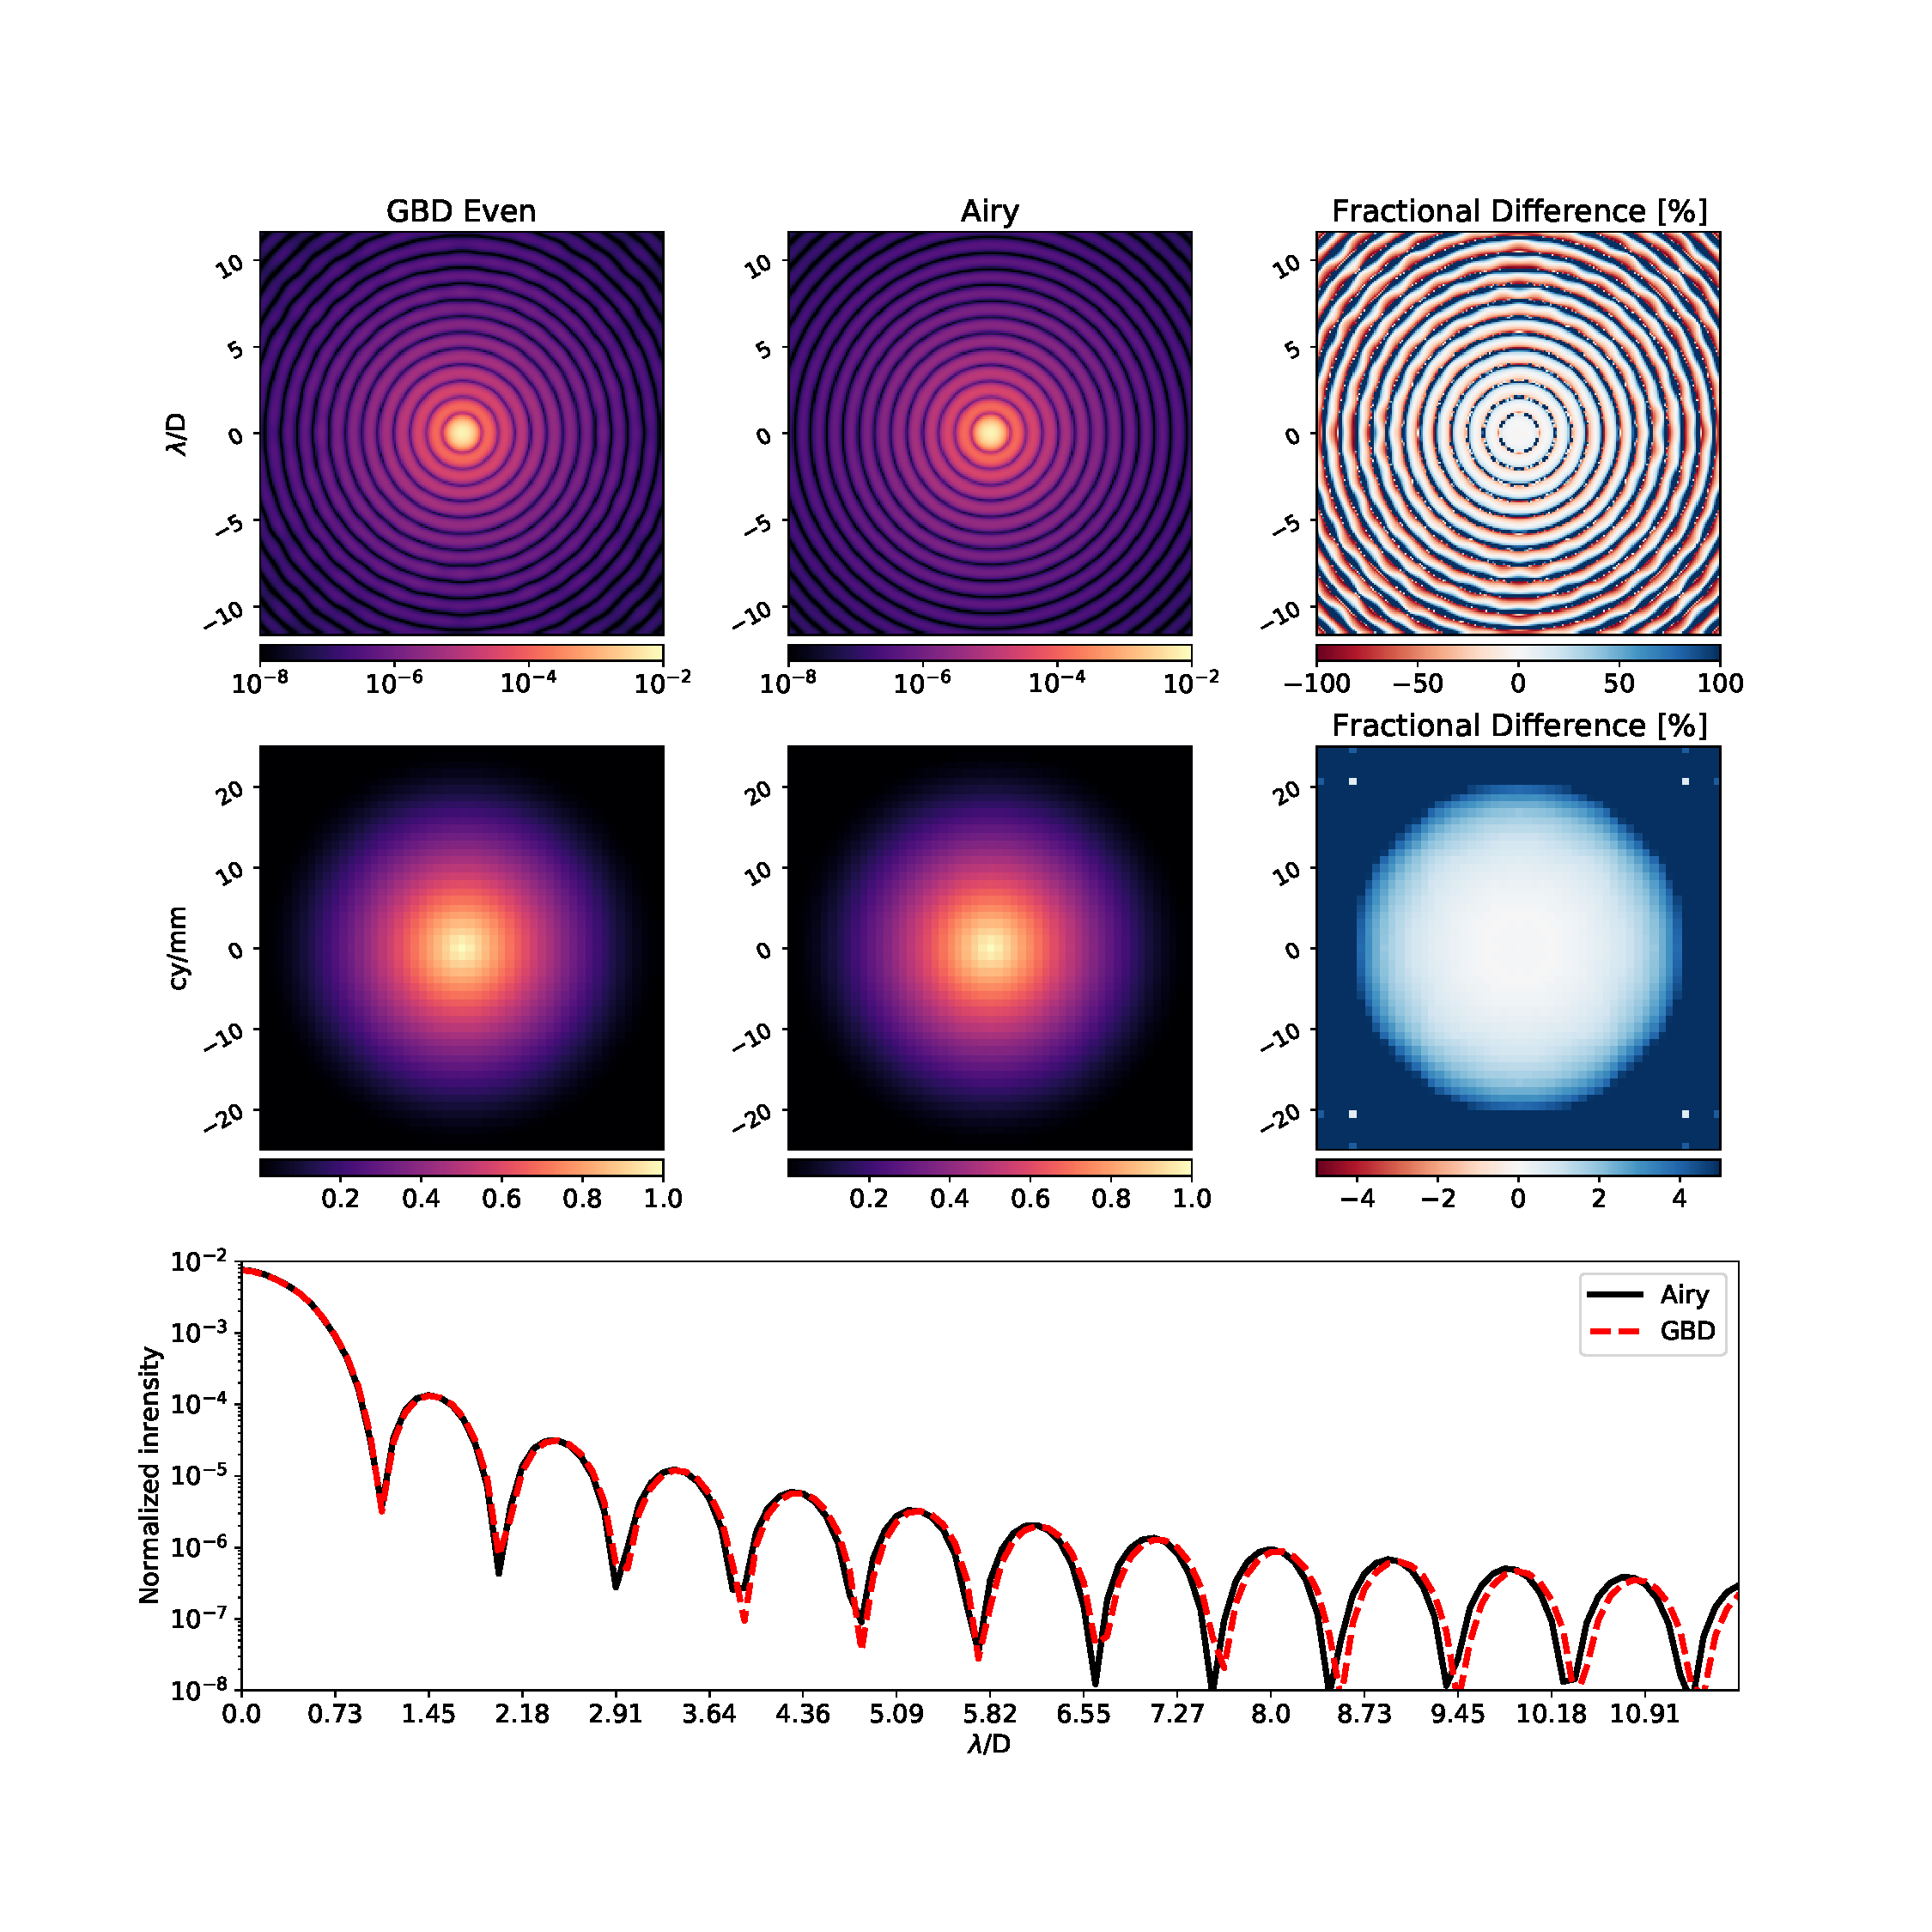
\includegraphics[width=\textwidth]{Airy_compare_Even.pdf}
    \caption{Comparisons of the PSF (top) and MTF (middle) for GBD with even sampling (left) and analytical Airy pattern (middle). The PSFs are given in units of normalized intensity, such that the sum of the energy in the PSF is unity. The fractional difference is plotted on the right, and the azimuthally averaged radial profile is plotted on the bottom. The MTF is plotted out to the cutoff frequency of the HST of around 25 cy/mm. The radial oscillation in the fractional difference PSF is indicative of the artifacts introduced by GBD. In the MTF it is apparent that frequencies below 20 cy/mm are well-maintained, but the higher spatial frequencies increase in fractional difference. The effect on the PSF is revealed in the radial profile, where the PSF appears to spread out at larger angular separations. The RMS difference of the PSF data is 2.3e-6.}
    \label{fig:airy_even}
\end{figure}

\begin{figure}[H]
    \centering
    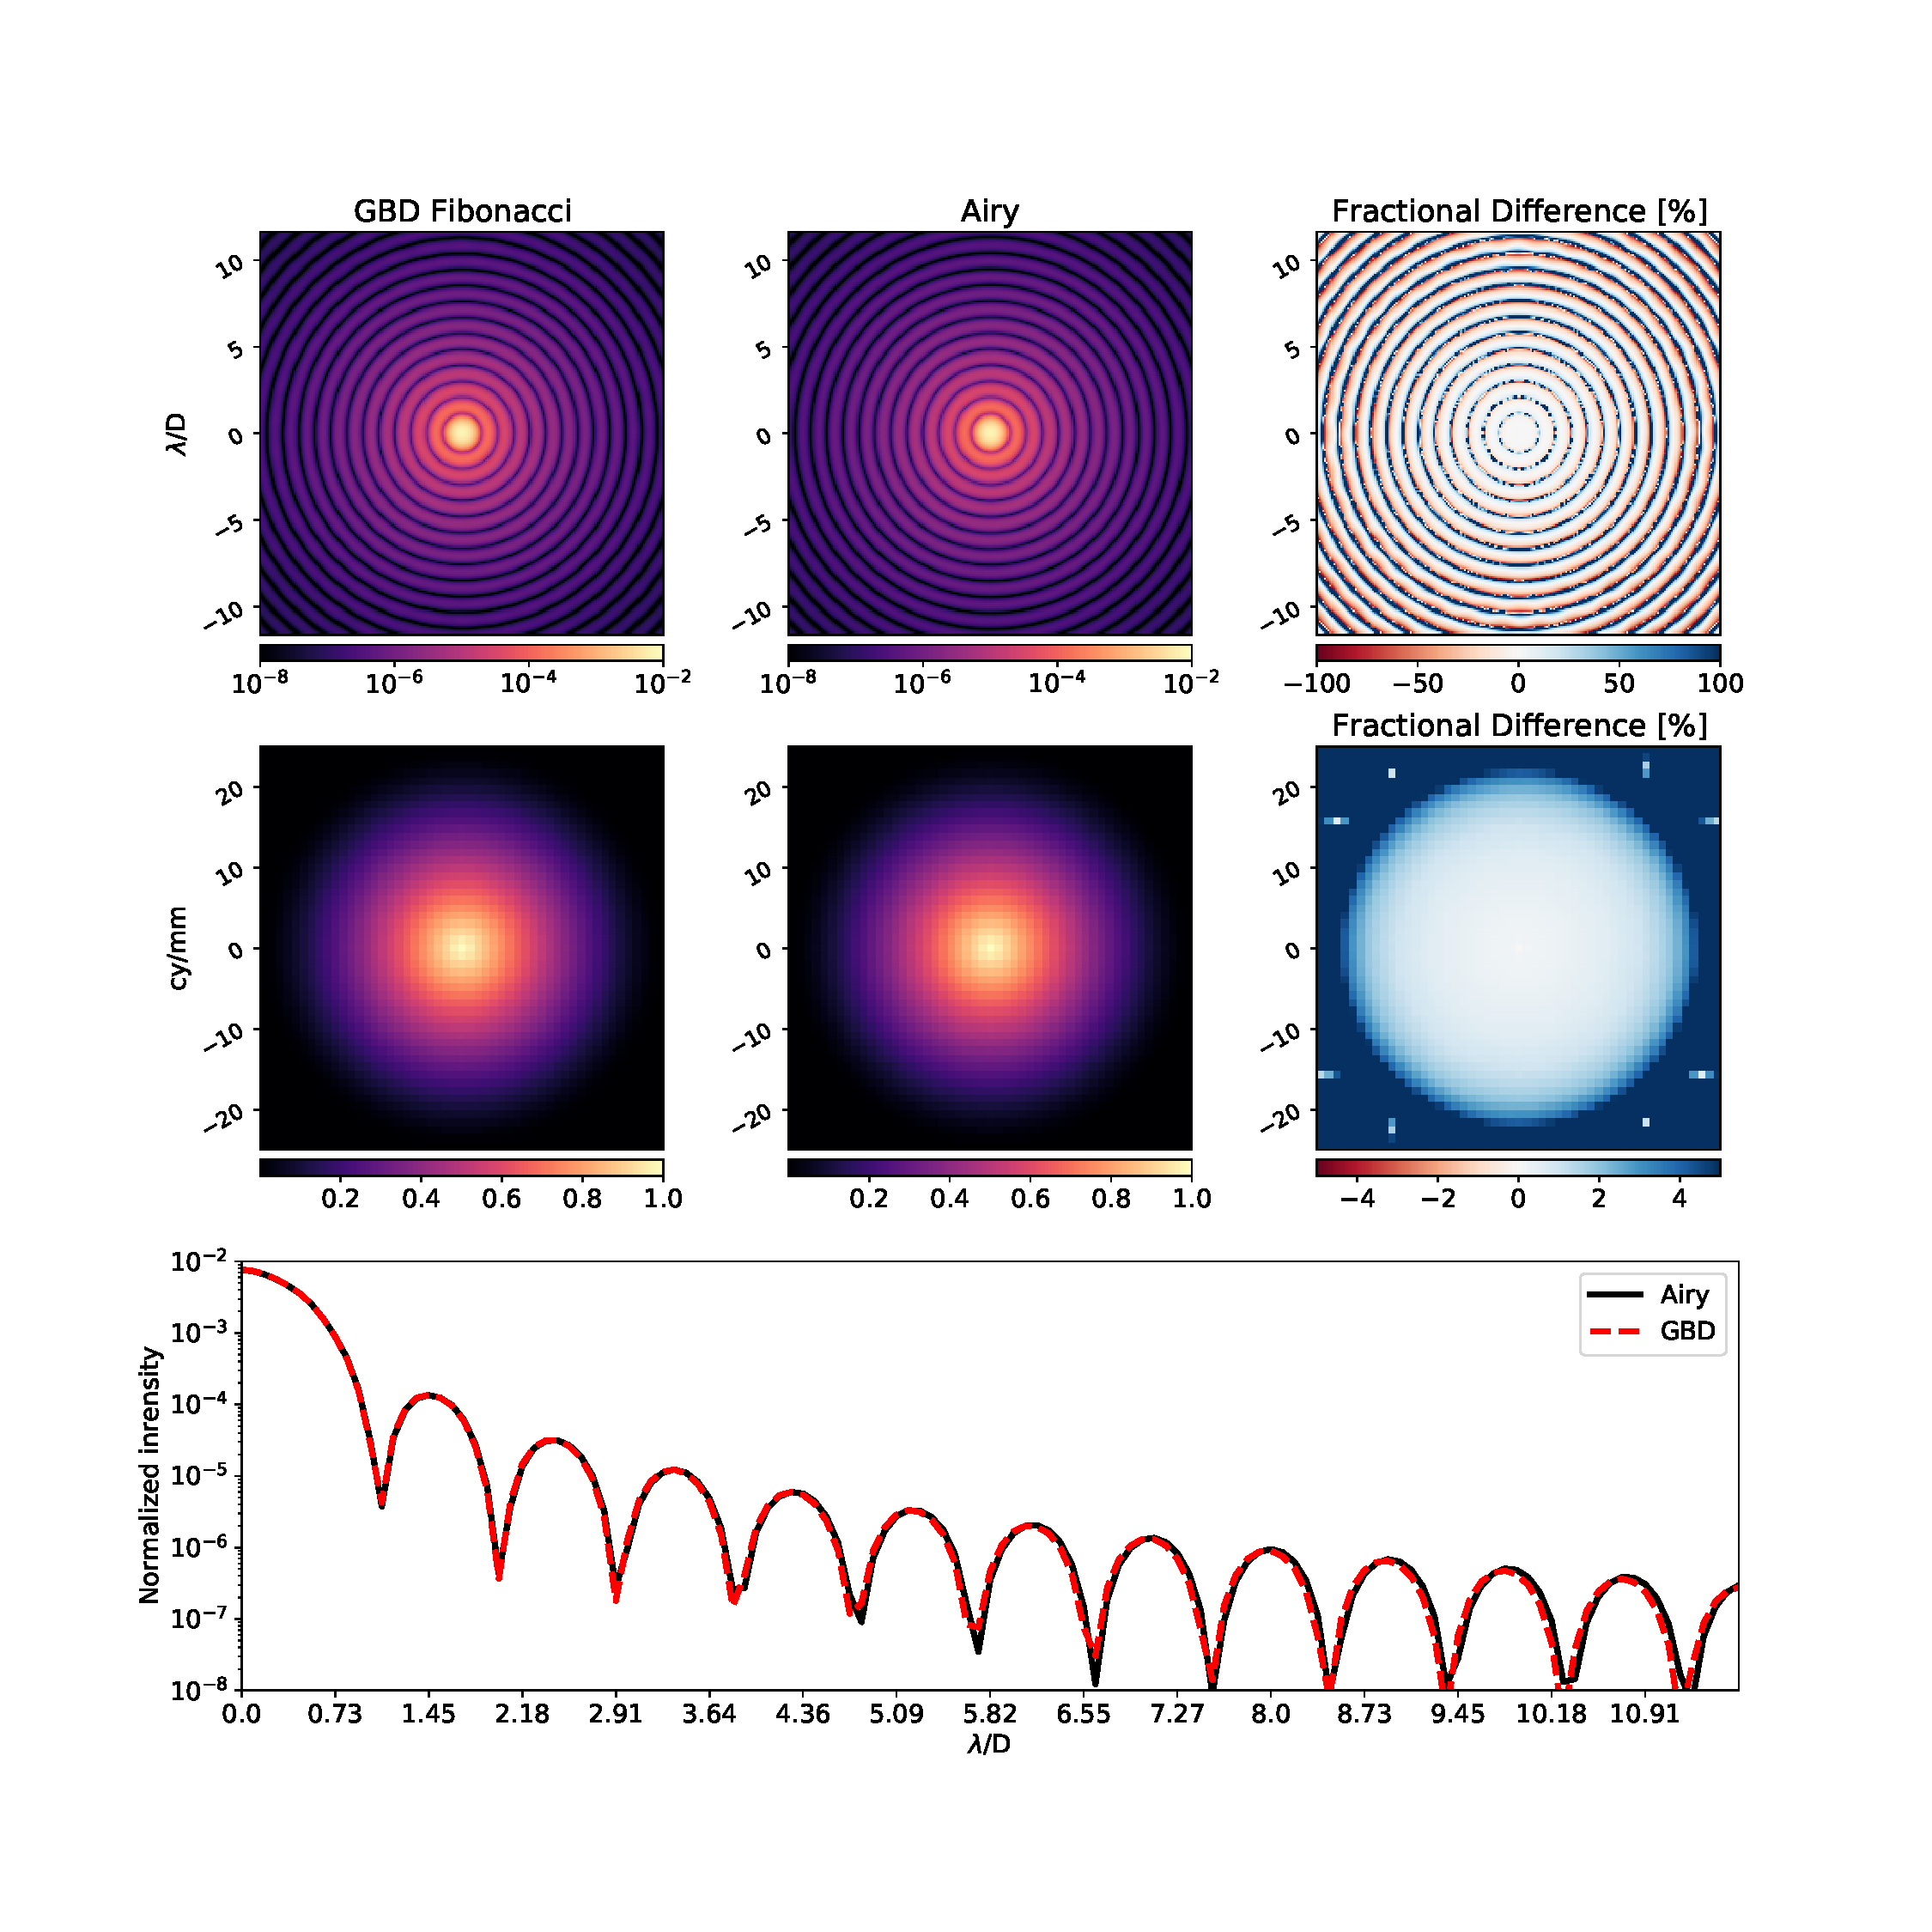
\includegraphics[width=\textwidth]{Airy_compare_Fib.pdf}
    \caption{Comparisons of the PSF (top) and MTF (middle) for GBD with Fibonacci sampling for the same number of beamlets as Figure \ref{fig:airy_even} (left) and analytical airy pattern (middle). The PSFs are given in units of normalized intensity, such that the sum of the energy in the PSF is unity. The fractional difference is plotted on the right, with the MTF plotted out to the cutoff frequency of the HST of around 25 cy/mm. The azimuthally averaged radial profile is plotted on the bottom. The presence of ripples in the fractional difference PSF is noticeably lower than Figure \ref{fig:airy_even}, and the fractional difference MTF shows that frequencies out to 23 cy/mm are well-maintained. The spreading present in Figure \ref{fig:airy_even} is less prevalent in the radial profile. The RMS difference of the PSF data is 1.6e-6, indicating that this distribution results in a more accurate simulation.}
    \label{fig:airy_fib}
\end{figure}

Figures \ref{fig:airy_even} and \ref{fig:airy_fib} compare the same simulation of the Airy function where the only variable is how the entrance pupil was decomposed. In both the PSF and MTF dimensions it is clear that the Fibonacci sampling is the superior decomposition method for this aperture. For more under-sampled cases there may be a tradeoff in accuracy. To understand this, in Figure \ref{fig:rms_vs_sample_airy} we examine how well the analytical Airy function is reconstructed for the two sample schemes as a function of the number of beamlets.

\begin{figure}[H]
    \centering
    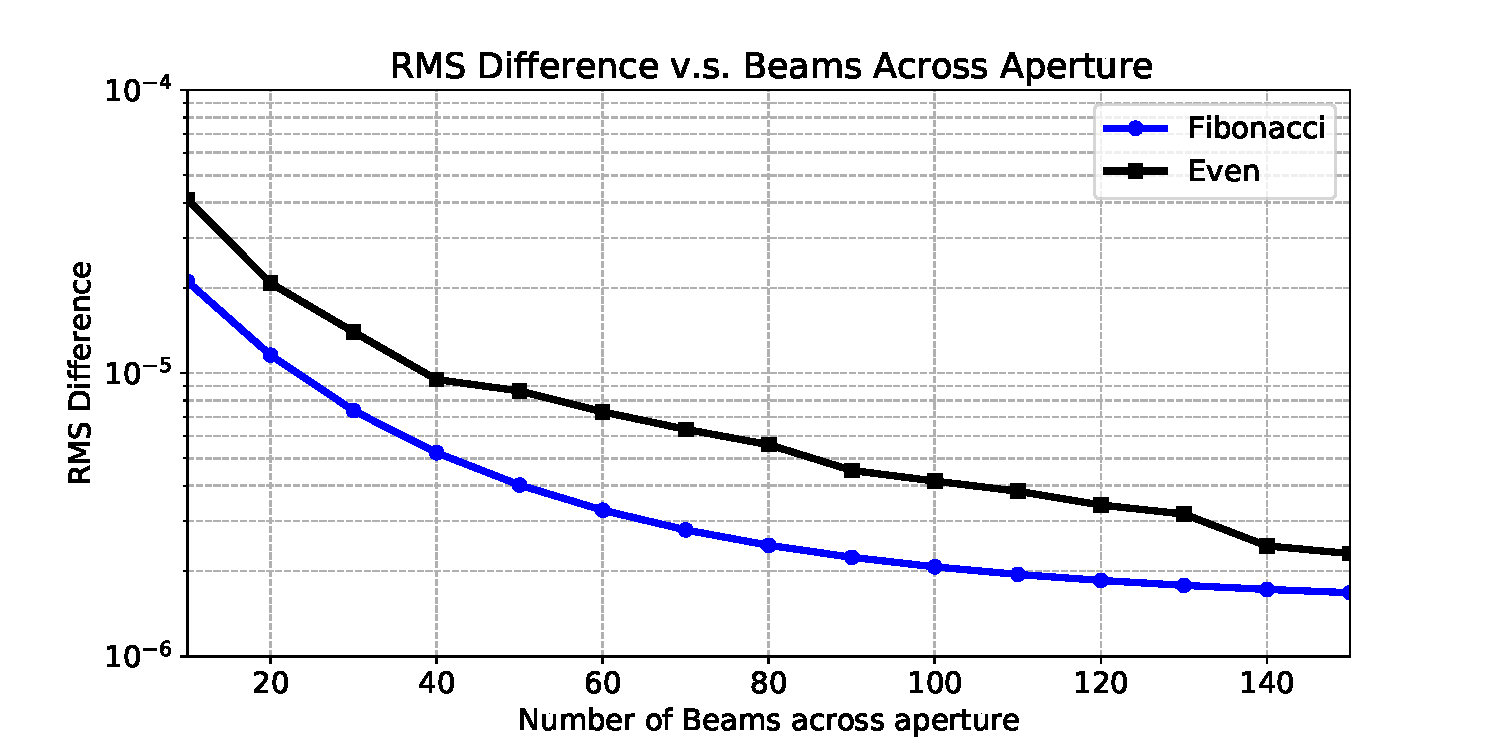
\includegraphics[width=\textwidth]{rms_vs_nbeamlets.pdf}
    \caption{The RMS difference between the sum-normalized GBD PSF and analytical Airy function for the Fibonacci (blue circles) and Even (black squares) sample schemes. For the circular aperture it is clear that the Fibonacci sample scheme is more accurate for every case given a circular aperture. However, the returns are diminishing as the number of beamlets increases.} 
    \label{fig:rms_vs_sample_airy}
\end{figure}

The Fibonacci sampling clearly wins out in terms of performance given a fixed number of beamlets, which translates directly to computation time. This also means that using the Fibonacci sample scheme can yield a simulation of the same accuracy as the even sample scheme with fewer beamlets. By judicious choice in sample scheme, the computational complexity of GBD can be lessened or the simulation accuracy can be increased.

To further test GBD's capability to model a more realistic observatory PSF, we add obscurations in the entrance pupil that correspond to the secondary mirror and supporting spiders. We also tilt the secondary mirror by 0.05 degrees to aberrate the beam. By doing so, we simultaneously test our algorithm's ability to capture aberrations from optical misalignment and diffraction from structure in the aperture. The results of this simulation are shown in Figure \ref{fig:aberrated}.

\begin{figure}[H]
    \centering
    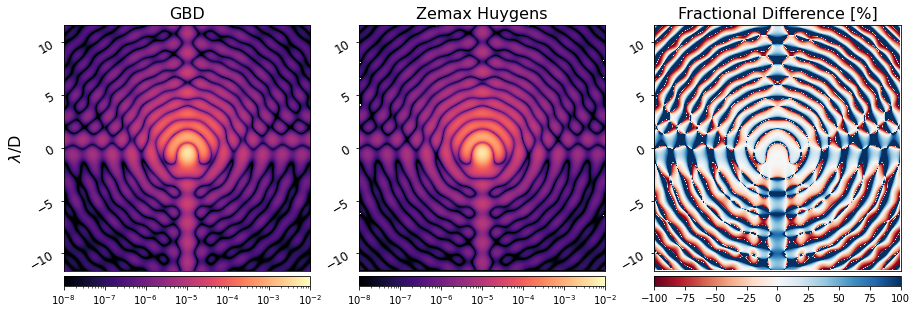
\includegraphics[width=0.9\textwidth]{hst_aberrated_psf.png}
    \caption{Simulations of an aberrated PSF with secondary support structure in the entrance pupil of our HST model given in Table \ref{tab:fiducial_observatory_specs}. The GBD PSF (left) and Zemax Huygens PSF (middle) have very similar structure, with the dominant difference in structure being the features from the sharp-edge diffraction from the spiders (shown in fractional difference on the right). This simulation helps quantify GBD's difficulty in modeling sharp-edge diffraction effects. The RMS difference of the PSF data is 7.5e-6.}
    \label{fig:aberrated}
\end{figure}

The data in Figure \ref{fig:aberrated} was simulated in a comparison between our proposed algorithm and Zemax's Huygens PSF analysis tool. The Huygens PSF is computed by propagating spherical waves along ray paths in Zemax to the image plane and coherently summing them. The Zemax documentation asserts that this method makes fewer assumptions than the FFT PSF, so it was chosen as the point of comparison for the aberrated PSF. In our GBD simulation we vignette any Gaussian Beam that has any of its differential rays vignetted. Our results show extremely similar structure in the PSF from both the aberration induced by the secondary mirror misalignment and the structure from the HST spiders. The fractional difference reveals that the first couple ``rings" of the PSFs are almost identical, indicating that the low-order aberrations were sufficiently simulated by GBD. There is a larger fractional difference in the dimmer structures that result from the sharp edges of the secondary obscuration and spiders, which is a known challenge for GBD simulations. This result can be further improved by careful implementation of alternative beamlet profiles, such as Worku and Gross's truncated beamlets\cite{Worku19}, or higher-order transverse electric field modes (e.g. Hermite, Laguerre-Gaussian). However, the result using fundamental Gaussian modes is encouraging, since the RMS difference of the PSFs is within the same order of magnitude as the results shown in Figures \ref{fig:airy_even} and \ref{fig:airy_fib}. Zemax is an industry standard optical modeling tool, but its propagation algorithms are closed-source. It is beyond the scope of this paper to validate the accuracy of Zemax's PSF simulation tools, but it is encouraging that our results in Figure \ref{fig:aberrated} agree. Now that our algorithm's ability to perform PSF simulations has been verified, we can analyze the degree to which it introduces artifacts in high-contrast imaging simulations.

\subsection{Coronagraph Response}
In traditional VCs, the on-axis field from an unvignetted circular aperture should be entirely rejected. We expect from the observatory PSF simulations that GBD does not trace high-spatial frequency information well due to the soft edges and amplitude ripples introduced by the beamlet decomposition. Any meaningful errors from this step should pass through the coronagraph unperturbed. To formally assess GBD's suitability for high-contrast imaging, we construct the PSF of the fiducial observatory with a circular aperture using GBD and compare it to a Fraunhofer model of the same system. Both PSFs are propagated with Fraunhofer diffraction through the vortex coronagraph and the coronagraph focal plane is compared to assess the presence, if any, of residual signal introduced by GBD. The parameters used in this simulation are given in Table \ref{tab:coro_params}, and the results shown in Figure \ref{fig:nonparaxial_coronagraph} are cropped to show the innermost 30 $\lambda / D$ to better display the structure near the inner working angle.

\begin{table}[H]
    \centering
    \begin{tabular}{c|c}
       \hline
       Parameter  & Value  \\
       \hline
        Wavelength ($\lambda$) & 1.65 $\mu$m \\
        Number of Pixels ($N_{pixels}$) & 1600 \\
        Instantaneous FoV ($\Delta x$) & 4.95 $\mu$m or $\frac{1}{8}\frac{\lambda}{D}$\\
       \hline
       \hline
    \end{tabular}
    \\
    \caption{Simulation parameters for the result shown in Figure \ref{fig:nonparaxial_coronagraph}. 
    }
    \label{tab:coro_params}
\end{table}

\begin{figure}[H]
    \centering
    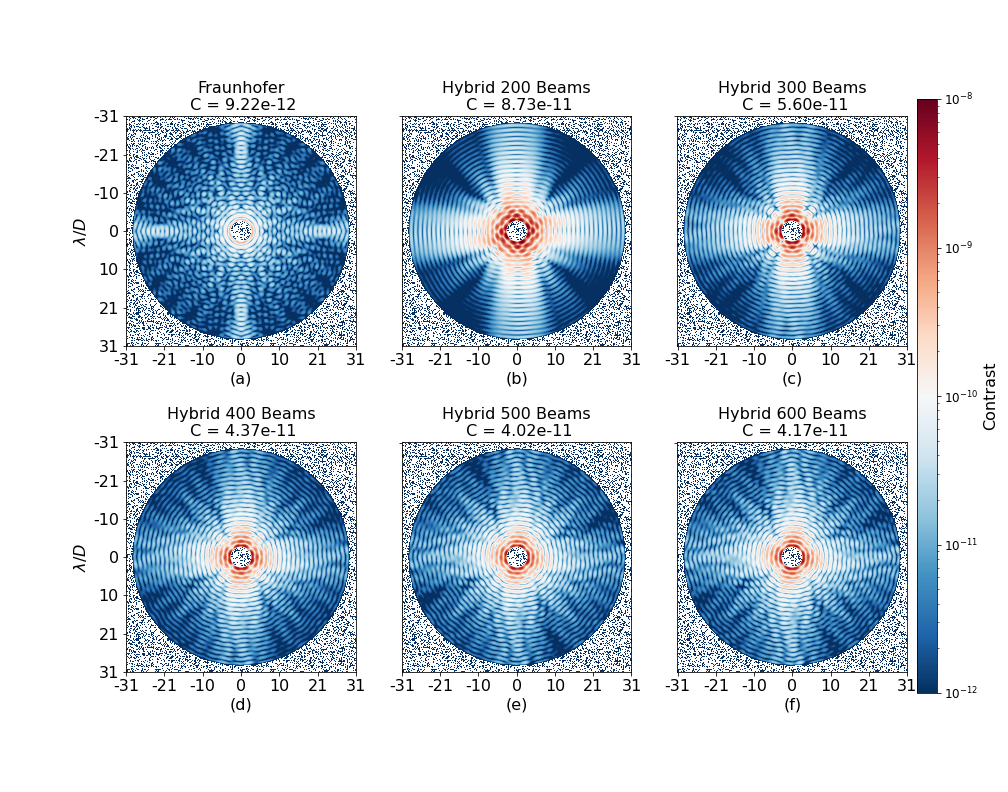
\includegraphics[width=0.9\textwidth, trim={3cm 0cm 2cm 0cm}]{coronagraph_vs_beamlets.png}
    \caption{Comparison of the coronagraph PSF from 3-30 $\lambda / D$ generated by a solely Fraunhofer diffraction model (a) and the proposed Hybrid propagation scheme for a varying number of beamlets across the 2.4m unobscured HST aperture with an overlap factor of 2. (b) was generated with 200 beamlets, (c) with 300 beamlets, (d) with 400 beamlets, (e) with 500 beamlets, and (f) with 600 beamlets across the aperture. These data were generated by producing a PSF with the given propagation scheme and then propagating it through HCIPy's VortexCoronagraph class with a topological charge of 2. To reflect the residual starlight's astrophysical flux ratio ``contrast", the PSF data are normalized to the maximum of an off-axis PSF at $\approx 16 \lambda/D$ that propagates through the VortexCoronagraph. The mean contrast of the masked region (C) is shown on each image. The residuals from the Hybrid propagation (b-f) are brighter than the equivalent Fraunhofer simulation, and minimize at the 500 beamlet case. This is particularly apparent near the inner working angle, where we see a maximum signal of $\approx$ $1 \times 10^{-8}$ for the 200 beamlet case decrease to $\approx 5 \times 10^{-9}$ in the 500 beamlet case.}
    \label{fig:nonparaxial_coronagraph}
\end{figure}

Figure \ref{fig:nonparaxial_coronagraph} shows the residuals that propagate through to the final image plane which arise from inaccuracies in the propagation model. The Hybrid propagation model generally minimizes in average contrast until the 600 beamlet case (Figure \ref{fig:nonparaxial_coronagraph}f) where there is a slight increase. The residuals from traditional Fraunhofer diffraction leave some low-energy features near the core of the PSF, which can be improved with greater sampling but the rest of the field is largely below $10^{-11}$ contrast. The decreasing residual energy with the number of beamlets used in the hybrid propagation scheme is encouraging, but we appear to have found the point at which increasing the number of Gaussian beams no longer increases simulation accuracy. 

The algorithm outlined in \hyperref[sec:algorithm]{Section \ref{sec:algorithm}} is carried out as-written with some computational acceleration done by taking advantage of Python's ability to vectorize matrix operations and other Python packages to accelerate the exponential calculation, discussed in detail in \hyperref[sec:appendixB]{Appendix B}. We have not formally explored parallel processing packages on Central Processing Units (CPUs) or Graphical Processing Units (GPUs) to accelerate this computation, but expect that these could make higher-sampled simulations more feasible to minimize the artifacts that remain in GBD PSFs for high-contrast imaging simulations.
Now that we have established an open-source platform for GBD, Worku's Modified GBD\cite{Worku19} could be developed to minimize the number of beamlets required to minimize the artifacts in the coronagraphic focal plane. Exploring higher order spatial modes and the astigmatic fundamental mode of Gaussian Beams could also yield greater accuracy for the same or less computational complexity. 
The result in Figure \ref{fig:nonparaxial_coronagraph} using traditional GBD shows that we can reduce the residuals to below $10^{-9}$ Contrast near the inner working angle. It is also worth noting that this result suggests that with sufficient sampling, GBD can presently be used to simulate the PSFs for systems with less stringent contrast floors. To minimize the residuals from the propagation technique, other decomposition methods must be explored. We have created a platform for the algorithm's development in an open-source environment and will outline a road map for the most pressing optimizations that can be conducted by future investigations to improve GBD's accuracy.

